\documentclass{beamer}


% Beamer settings
\usecolortheme{rose}
\beamertemplatenavigationsymbolsempty
\setbeamertemplate{footline}[frame number]

\titlegraphic{%

\includegraphics[height=1cm]{logo-full-colour.png}}

\addtobeamertemplate{frametitle}{}{%
\begin{tikzpicture}[remember picture,overlay]
\node[anchor=north east,yshift=2pt] at (current page.north east) {
\includegraphics[height=1cm]{logo-full-colour.png}};
\end{tikzpicture}}

% Packages
\usepackage{amsmath}

\usepackage{tikz}
\usetikzlibrary{positioning}
\usetikzlibrary{fit}

\usepackage{pgfplots}
\usepgfplotslibrary{fillbetween}

\usepackage{minted}
\usepackage[T1]{fontenc} % Required by minted to ensure dollar signs are produced instead of pound (sterling) signs

\usepackage{multicol}

\usepackage{booktabs}

\usepackage{adjustbox}

% Author
\author{Simon McIntosh-Smith \& Tom Deakin\\University of Bristol}

\date{}



\title{OpenMP for Computational Scientists}
\subtitle{4: Combining MPI and OpenMP}

\begin{document}

\frame{\titlepage}

%-------------------------------------------------------------------------------
\section{Outline}
\begin{frame}
\frametitle{Outline}

\begin{itemize}
  \item Quick recap
  \item Calculating memory bandwidth for the 5-point stencil code
\end{itemize}

\vfill

Programming beyond a single multi-core CPU:
\begin{itemize}
  \item Non-uniform Memory Access
  \item Thread affinity in OpenMP
  \item Combining MPI with OpenMP
\end{itemize}
\end{frame}

%-------------------------------------------------------------------------------
\section{Recap}
\begin{frame}
\frametitle{Recap}

We've already come a long way!

\begin{itemize}
  \item Parallelise loops with OpenMP: \mintinline{fortran}|!$omp parallel do|.
  \item Data sharing clauses.
  \item Synchronisation with barriers, atomics and \mintinline{fortran}|critical| regions.
  \item Reductions with the \mintinline{fortran}|reduction| clause.
  \item The cache hierarchy.
  \item Performance analysis and the Roofline model.
  \item Vectorisation along with the OpenMP \mintinline{fortran}|simd| construct.
  \item Optimisations for memory access.
\end{itemize}

\end{frame}

%-------------------------------------------------------------------------------
\begin{frame}[fragile]
\frametitle{Previous exercise}

Vectorise and optimise memory access patterns of your parallel 5-point stencil code:
\begin{minted}[frame=single,breaklines,fontsize=\scriptsize]{fortran}
!$omp parallel do reduction(+:total)
do j = 1, ny
  !$omp simd
  do i = 1, nx
    Atmp(i,j) = (A(i-1,j) + A(i+1,j) + A(i,j) + A(i,j-1) + A(i,j+1)) * 0.2
    total = total + Atmp(i,j)
  end do
  !$omp end simd
end do
!$omp end parallel do
\end{minted}

\begin{itemize}
  \item Swapped loops to ensure stride-1 access pattern.
  \item Removed division!
  \item Use \mintinline{fortran}|simd| construct on inner loop (removing \mintinline{fortran}|collapse| clause).
  \item Checked vectorisation report: assume sizes arrays cause issue, so move kernel into \mintinline{fortran}|subroutine|.
\end{itemize}

\end{frame}

%-------------------------------------------------------------------------------
\begin{frame}
\frametitle{Calculating memory bandwidth}
Is your 5-point stencil code \emph{fast}?

\pause

Calculate memory bandwidth of the \emph{kernel} as a whole:
\begin{itemize}[<+->]
  \item Assume a ``perfect cache'' model: once you read a memory location, it's been cached and further reads are ``free'' within the kernel.
  \item All of \mintinline{fortran}|A| array is read: $nx \times ny$ reads.
  \item All of \mintinline{fortran}{Atmp} array is written: $nx \times ny$ reads.
  \item Total memory moved: $2 \times nx \times ny \times 8$ bytes data moved (double precision) \emph{per iteration}.
  \item Memory bandwidth: $\frac{ntimes \times 2 \times nx \times ny \times 8}{runtime}$ bytes/second.
\end{itemize}


\end{frame}

%-------------------------------------------------------------------------------
\begin{frame}
\frametitle{Achieved memory bandwidth}

Results on dual-socket Intel Xeon E5-2680 v4 @ 2.40GHz, 14 cores/socket.
Compiled with Intel 2018 compiler, {\tt -O3 -xHost}.

\vfill

Set $nx=ny=20,000$ so arrays are 3.2~GB. Set $ntimes=30$. Removed \mintinline{fortran}|write| statement. Taken best of 5 runs.

\vfill

\pause
Theoretical peak bandwidth\footnote{\url{https://ark.intel.com/products/91754/Intel-Xeon-Processor-E5-2680-v4-35M-Cache-2_40-GHz}}: $2 \times 76.8 \text{GB/s} = 153.6 \text{GB/s}$. \\
STREAM Triad: 129.0~GB/s (84\% theoretical peak).

\pause
\begin{table}
\begin{tabular}{ccc}
\toprule
Version & Runtime (s) & Memory bandwidth (GB/s)\\
\midrule
Initial parallel reduction & 25.667 &  7.48 \\
Swap loops + vectorise     &  4.876 & 39.38 \\
\bottomrule
\end{tabular}
\end{table}

Achieving 30.5\% of STREAM memory bandwidth.

\end{frame}

%-------------------------------------------------------------------------------
\section{NUMA}
\begin{frame}
\frametitle{NUMA Architecture}

Recall this cartoon of a dual-socket, shared memory system:
\begin{center}
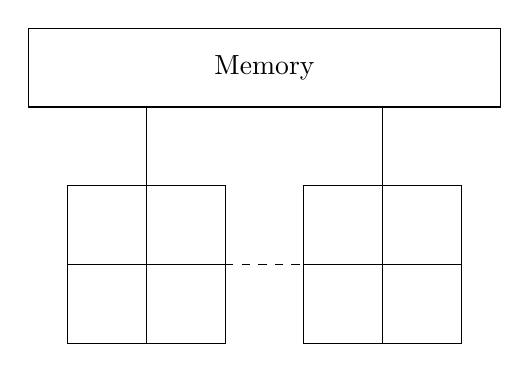
\begin{tikzpicture}
  % Draw 4 cores for socket 0
  \draw (0,0) rectangle (1,1);
  \draw (1,0) rectangle (2,1);
  \draw (0,1) rectangle (1,2);
  \draw (1,1) rectangle (2,2);

  % Draw 4 cores for socket 1
  \draw (3,0) rectangle (4,1);
  \draw (4,0) rectangle (5,1);
  \draw (3,1) rectangle (4,2);
  \draw (4,1) rectangle (5,2);

  % Draw large memory
  \draw (-0.5,3) rectangle (5.5,4);
  \draw (2.5,3.5) node {Memory};

  % Connect sockets to memory
  \draw (1,2) -- (1,3);
  \draw (4,2) -- (4,3);
  \draw[dashed] (2,1) -- (3,1); % QPI

\end{tikzpicture}
\end{center}

\emph{All} threads (each running on a core) can access the same memory.

\end{frame}
%-------------------------------------------------------------------------------

\begin{frame}
\frametitle{NUMA Architecture}
\begin{itemize}
  \item In reality on a dual-socket system each \emph{socket} is physically connected to half of the memory.
  \item Still shared memory: all cores can access all the memory.
  \item A core in the first socket wanting memory attached to the other socket must:
    \begin{itemize}
      \item Go via the socket-to-socket interconnect.
      \item Access memory via the other socket's memory controllers.
    \end{itemize}
  \item Accessing memory from other socket is slower than access from own socket.
\end{itemize}
\begin{center}
\resizebox{!}{3.5cm}{
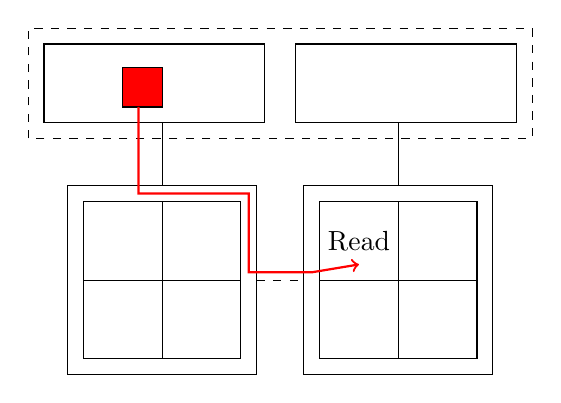
\begin{tikzpicture}
  % Draw 4 cores for socket 0
  \foreach \i in {0,1,3,4} {
    \foreach \j in {0, 1} {
      \draw (\i,\j) rectangle (\i+1,\j+1);
    }
  }

  % Draw sockets around cores
  \draw (-0.2, -0.2) rectangle (2.2, 2.2);
  \draw (2.8, -0.2) rectangle (5.2, 2.2);

  % Draw large memory
  \draw (-0.5,3) rectangle (2.3,4);
  \draw (2.7,3) rectangle (5.5,4);
  \draw[dashed] (-0.7,2.8) rectangle (5.7,4.2);

  % Connect sockets to memory
  \draw (1,2.2) -- (1,3);
  \draw (4,2.2) -- (4,3);
  \draw[dashed] (2.2,1) -- (2.8,1); % QPI

  % Show memory shared
  \pause
  \draw[fill=red] (0.5,3.2) rectangle (1,3.7);
  \draw (3.5,1.5) node {Read};
  \pause
  \draw[->,red,thick] (0.7,3.2) -- (0.7,2.1) -- (2.1,2.1) -- (2.1,1.1) -- (2.9,1.1) -- (3.5,1.2);

\end{tikzpicture}
}
\end{center}
\end{frame}

%-------------------------------------------------------------------------------
\begin{frame}
\frametitle{Memory allocation}
\begin{itemize}
  \item What happens when you run \mintinline{fortran}|allocate(A(1:N))|?
  \pause
  \item Allocating memory does not necessarily allocate memory!
  \item Memory is allocated when it's first used (i.e. \mintinline{fortran}|A(i) = 1.0|), one \emph{page} at a time.
  \item OS tends to use a \emph{first touch policy}.
  \item Memory is allocated in the closest NUMA region to the thread that first touches the data.
  \item Ideally want threads to use data in local NUMA region to reduce socket-to-socket interconnect transfers.
\end{itemize}
\end{frame}

%-------------------------------------------------------------------------------
\subsection{First touch}
\begin{frame}[fragile]
\frametitle{Taking advantage of first touch}
Parallelising your data initialisation routine might mean your main loops go faster!


\begin{minted}[fontsize=\small,linenos,frame=single]{fortran}
! Allocate and initialise vectors
allocate(A(N), B(N), C(N))
!$omp parallel do
do i = 1, N
  A(i) = 1.0
  B(i) = 2.0
  C(i) = 0.0
end do
!$omp end parallel do

! Vector add
!$omp parallel do
do i = 1, N
  C(i) = A(i) + B(i)
end do
!$omp end parallel do
\end{minted}

\end{frame}

%-------------------------------------------------------------------------------
\begin{frame}
\frametitle{NUMA-aware}
\begin{itemize}
  \item Parallelise your initialisation routines the same way you parallelise the main loops.
  \item This means each thread touches the same data in initialisation and compute.
  \item Should reduce the number of remote memory accesses needed and improve run times.
  \item But, OS is allowed to move threads around cores, and between sockets.
  \item This will mess up your NUMA aware code!
\end{itemize}
\end{frame}

%-------------------------------------------------------------------------------
\section{Thread affinity}
\begin{frame}
\frametitle{Pinning threads}
\begin{itemize}
  \item OpenMP gives you the controls to pin threads to specific cores.
  \item Exposed as \emph{places} and \emph{thread pinning policy} to those places.
  \item By default there is one place consisting of all the cores.
  \item Use the \mintinline{bash}|OMP_PROC_BIND| environment variable to set pinning for all \mintinline{fortran}|parallel| regions.
  \item Can use the \mintinline{bash}|proc_bind| clause for control of specific regions, but advise against this.
\end{itemize}
\end{frame}

%-------------------------------------------------------------------------------
\begin{frame}
\frametitle{OMP\_PROC\_BIND}
\begin{itemize}
  \item \mintinline{bash}|OMP_PROC_BIND=false|: Often the default; threads may move! \mintinline{fortran}|proc_bind| clauses ignored.
  \item \mintinline{bash}|OMP_PROC_BIND=true|: Threads won't move, and follow \mintinline{fortran}|proc_bind| clauses or else the implementation default pinning.
  \item \mintinline{bash}|OMP_PROC_BIND=master|: Threads pinned to same place as master thread.
  \item \mintinline{bash}|OMP_PROC_BIND=close|: Threads are assigned to places close to the master thread.
  If \mintinline{bash}|OMP_NUM_THREADS.eq.ncores|: thread 0 will pin to core 0; thread 1 will pin to core 1; etc
  \item \mintinline{bash}|OMP_PROC_BIND=spread|: Threads are assigned to places ``sparsely''.
  If \mintinline{bash}|OMP_NUM_THREADS.eq.ncores|: thread 0 will pin to socket 0 core 0; thread 1 will pin to socket 1 core 0; thread 2 will pin to socket 0 core 1; etc.
\end{itemize}
\end{frame}

%-------------------------------------------------------------------------------
\begin{frame}
\frametitle{Places}
\begin{itemize}
  \item The affinity (policy) defines how threads are assigned to places.
  \item Places allow you to divide up the hardware resource, so that threads can be assigned to them.
  \item Default: one place with all cores.
  \item Use \mintinline{bash}|OMP_PLACES| environment variable to control.
  \item \mintinline{bash}|OMP_PLACES=thread|: each place is a single hardware thread.
  \item \mintinline{bash}|OMP_PLACES=cores|: each place is a single core (containing one or more hardware threads).
  \item \mintinline{bash}|OMP_PLACES=sockets|: each place contains the cores of a single socket.
  \item Can also use list notation: \mintinline{bash}|OMP_PLACES="{0:4},{4:4},{8:4},{12:4}"|
\end{itemize}
\end{frame}

%-------------------------------------------------------------------------------
\begin{frame}
\frametitle{Thread pinning summary}
\begin{itemize}
  \item In general, going to want to just use \mintinline{bash}|OMP_PROC_BIND=true|.
  \item Sometimes \mintinline{bash}|spread| or \mintinline{bash}|close| gets better performance.
  \item Pinning rules can get complicated when there are multiple places, so prefer to use the predefined values.
  \item Most effective with a NUMA-aware implementation.
  \item Also helps reduce run-to-run timing variability.
  \item But must be careful with MPI+OpenMP pinning: more on this later\dots
\end{itemize}
\end{frame}

%-------------------------------------------------------------------------------
\section{Hybrid MPI and OpenMP}
\begin{frame}
\frametitle{Why combine MPI+OpenMP}
\begin{itemize}
  \item Supercomputers are often constructed with a hierarchical structure:
    \begin{itemize}
      \item Shared memory nodes connected with a network.
    \end{itemize}
  \item Need MPI (or similar) to communicate between distribued nodes.
  \item With multi-core, could just run MPI everywhere (flat MPI).
  \item But there are advantages to running \emph{hybrid} MPI and OpenMP:
    \begin{itemize}
      \item Larger fewer messages to take advantage of network bandwidth.
      \item Fewer MPI ranks to manage (fewer to synchronise and for collectives).
      \item Can avoid memory copies for intra-node communication.
      \item Reduced memory footprint.
      \item Parallelise other problem dimensions not decomposed with MPI.
    \end{itemize}
\end{itemize}
\end{frame}

%-------------------------------------------------------------------------------
\begin{frame}
\frametitle{Scaling}
\begin{itemize}
  \item Strong scaling:
    \begin{itemize}
      \item Take a fixed problem and add more compute resource.
      \item Would hope runtime reduces with more resource.
    \end{itemize}
  \item Weak scaling:
    \begin{itemize}
      \item Take a fixed problem \emph{per compute resource}, and add more resource.
      \item Problem gets bigger with more resources.
      \item Would hope runtime stays constant.
    \end{itemize}
  \item In both cases, typically see scaling of MPI-only codes tail off at high node counts.
  \item Hybrid MPI+OpenMP codes often continue scaling.
\end{itemize}
\end{frame}


%-------------------------------------------------------------------------------
\begin{frame}[fragile]
\frametitle{MPI programs}
What happens when you run an MPI program?
\begin{minted}{bash}
mpirun -np 16 ./a.out
\end{minted}

\begin{itemize}
  \item 16 processes are spawned on one (or more) nodes according to the hostname list file given by the queuing system.
    \begin{itemize}
      \item E.g. with PBS (\mintinline{bash}|qsub|, etc.) set by \mintinline{bash}|$PBS_NODEFILE|.
    \end{itemize}
  \item There is no reason why these processes have to be serial:
  \begin{itemize}
    \item Each MPI rank could spawn OpenMP threads and run in parallel.
    \item Each MPI rank could use a GPU.
  \end{itemize}
\end{itemize}

\end{frame}

%-------------------------------------------------------------------------------
\begin{frame}[fragile]
\frametitle{Compiling OpenMP and MPI code}
\begin{itemize}
  \item Remember building MPI code just uses the wrapper commands.
  \item Just pass in the OpenMP flag as usual:
    \begin{itemize}
      \item GNU: \mintinline{bash}|mpif90| -fopenmp
      \item Intel: \mintinline{bash}|mpiifort| -qopenmp
      \item Cray: \mintinline{bash}|ftn|
    \end{itemize}
  \item Set the number of OpenMP threads \emph{per rank}.
  \item E.g 2 MPI ranks, 8 threads per rank:
  \begin{minted}{bash}
  OMP_NUM_THREADS=8 mpirun -np 2 ./a.out
  \end{minted}
\end{itemize}
\end{frame}

%-------------------------------------------------------------------------------
\begin{frame}[fragile]
\frametitle{Combining OpenMP and MPI}
\begin{itemize}
  \item MPI assumes that each MPI process does not spawn anything else.
  \item Must initialise MPI differently if using threads!
  \begin{minted}{fortran}
  call MPI_Init_thread(required, provided, ierr)
  \end{minted}

  \item You specify a required thread support level, and it returns the level it could support.
  \item A good idea to check \mintinline{fortran}|provided .ge. required|.
\end{itemize}
\end{frame}

%-------------------------------------------------------------------------------
\begin{frame}
\frametitle{Thread support levels}
\begin{itemize}
  \item \mintinline{fortran}|MPI_THREAD_SINGLE| \\
  Only one thread will execute (no threads allowed).

  \item \mintinline{fortran}|MPI_THREAD_FUNNELED| \\
  May spawn threads, but only the original process may call MPI routines: the one that called \mintinline{fortran}|MPI_Init|.

  \item \mintinline{fortran}|MPI_THREAD_SERIALIZED| \\
  May spawn threads and any thread can make MPI calls, but only one at a time. \emph{Your} responsibility to synchronise.

  \item \mintinline{fortran}|MPI_THREAD_MULTIPLE| \\
  May spawn threads and any thread can make MPI calls. The MPI library has to deal with being called in parallel.
\end{itemize}

Remember to make sure ranks still match the MPI communications to avoid deadlock.

\end{frame}

%-------------------------------------------------------------------------------
\begin{frame}[fragile]
\frametitle{Example: MPI\_THREAD\_FUNNELED}
Only the original process is allowed to call MPI routines.
\begin{minted}[frame=single]{fortran}
!$omp parallel
... ! Parallel work
!$omp end parallel
call MPI_Sendrecv()
\end{minted}
\end{frame}

%-------------------------------------------------------------------------------
\begin{frame}[fragile]
\frametitle{MPI\_THREAD\_SERIALIZED}
The threads are allowed to call MPI, but you must program in synchronisation to ensure only one thread calls MPI at a time.
\begin{minted}[frame=single]{fortran}
!$omp parallel
  ... ! Parallel work
  !$omp critical
  call MPI_Sendrecv()
  !$omp end critical
!$omp end parallel
\end{minted}
\end{frame}

%-------------------------------------------------------------------------------
\begin{frame}[fragile]
\frametitle{MPI\_THREAD\_MULTIPLE}
Any thread can call MPI whenever it likes. The \mintinline{fortran}|MPI_THREAD_MULTIPLE| guarantees the MPI library will be OK with this.
\begin{minted}[frame=single]{fortran}
!$omp parallel
  ... ! Parallel work
  call MPI_Sendrecv()
!$omp end parallel
\end{minted}
\end{frame}

%-------------------------------------------------------------------------------
\subsection{Hybrid thread pinning}
\begin{frame}
\frametitle{Thread pinning}
\begin{itemize}
  \item Need to be very careful how MPI ranks and OpenMP threads are mapped to the physical hardware.
  \item Imagine 2 dual-socket nodes: 4 sockets with (say) 16 cores per socket.
  \item Launch 64 MPI ranks: 1 per core.
    \begin{itemize}
      \item This is flat MPI.
      \item Launching OpenMP threads will over-allocate threads compared to hardware resource.
      \item Warning: things will slow down.
    \end{itemize}
  \item Launch 4 MPI ranks (one per socket).
    \begin{itemize}
      \item Leaves 16 cores per MPI rank for OpenMP threads to run on.
      \item But need to make sure processes \emph{and} threads go to the right places!
      \item Often close interaction with the queuing system --- system dependant behaviour.
    \end{itemize}
\end{itemize}
\end{frame}

%-------------------------------------------------------------------------------
\begin{frame}[fragile]
\frametitle{Example: default placement}
Example MPI rank placement with standard PBS setup.

Job requested 2 nodes.

\begin{minted}{bash}
mpirun -np 4 ./a.out
\end{minted}

\begin{center}
\begin{adjustbox}{max width={\textwidth}}
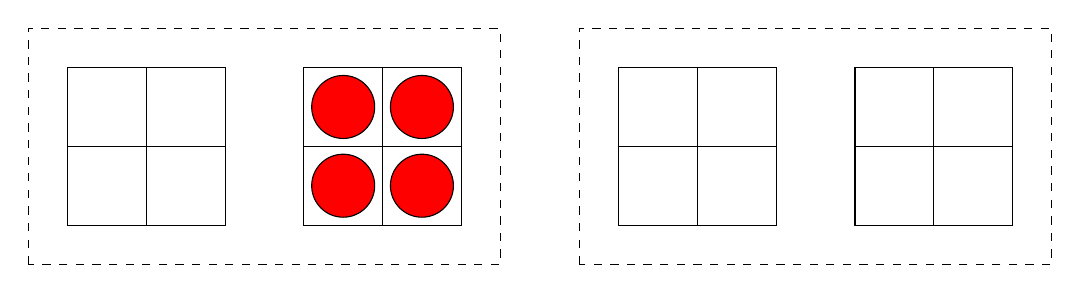
\begin{tikzpicture}

  \foreach \loc in {0, 3, 7, 10} {
  \foreach \i in {0,...,1} {
    \foreach \j in {0,...,1} {
      \draw (\loc+\i,\j) rectangle (\loc+\i+1,\j+1);
    }
  }
  }

  \draw[dashed] (-0.5,-0.5) rectangle (5.5,2.5);
  \draw[dashed] (6.5,-0.5) rectangle (12.5,2.5);

  \foreach \i in {0,...,1} {
    \foreach \j in {0,...,1} {
      \draw<2->[fill=red] (3+\i+.5,\j+.5) circle (0.4cm);
    }
  }
\end{tikzpicture}
\end{adjustbox}
\end{center}
\onslide<2->{
 All ranks placed on the second socket of the first node.
}
\end{frame}

%-------------------------------------------------------------------------------

\begin{frame}[fragile]
\frametitle{Example: pin MPI to one core per socket}
\begin{itemize}
  \item Tell the OS and MPI runtime to pin each MPI to the first core in each socket.
  \item Then want to launch 4 OpenMP threads per process.
  \item For OpenMPI:
  \begin{minted}{bash}
  export OMP_NUM_THREADS=4
  mpirun -np 4 --npersocket 1 ./a.out
  \end{minted}
  \item Where do the threads go?
\end{itemize}


\begin{center}
\begin{adjustbox}{max width={\textwidth}}
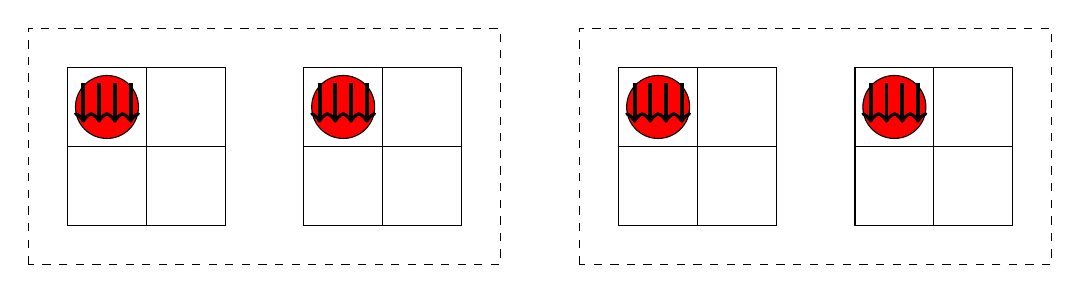
\begin{tikzpicture}

  \foreach \loc in {0, 3, 7, 10} {
  \foreach \i in {0,...,1} {
    \foreach \j in {0,...,1} {
      \draw (\loc+\i,\j) rectangle (\loc+\i+1,\j+1);
    }
  }
  }

  \draw[dashed] (-0.5,-0.5) rectangle (5.5,2.5);
  \draw[dashed] (6.5,-0.5) rectangle (12.5,2.5);

  \foreach \i in {0, 3, 7, 10} {
    \draw[fill=red] (\i+0.5,1.5) circle (0.4cm);
    \foreach \j in {0.2, 0.4, 0.6, 0.8} {
      \draw<2->[->,line width=.5mm] (\i+\j,1.8) -- (\i+\j, 1.3);
    }
  }
\end{tikzpicture}
\end{adjustbox}
\end{center}

\onslide<2->{
Threads spawned inherit their parent's binding, which was one core.

Use \mintinline{bash}|--report-bindings| flag to see what's being pinned where.

}

\end{frame}

%-------------------------------------------------------------------------------
\begin{frame}
\frametitle{Example: pin MPI to socket}
\begin{itemize}
  \item Pin each MPI process to the cores of a socket.
  \item MPI process \emph{could} move around those cores.
  \item OpenMP threads can spawn across the socket.
  \item OpenMPI gives three ways to do this:
  \begin{itemize}
    \item \mintinline{bash}|--bind-to-socket|
    \item \mintinline{bash}|--bind-to-core --cpus-per-proc 8|
    \item \mintinline{bash}|--map-by socket:PE=8| (v1.10 and up)
  \end{itemize}
\end{itemize}
\end{frame}

%-------------------------------------------------------------------------------
\begin{frame}
\frametitle{Pinning with Intel and Cray}
\begin{itemize}
  \item Intel MPI will need different flags and environment variables, but tends to do the right thing by default.
  \item Cray MPI (MVAPICH) can be controlled using \mintinline{bash}|aprun|.
    \begin{itemize}
      \item Use the \mintinline{bash}|-d| flag to specify the threads per process.
      \item Pinning usually happens correctly.
    \end{itemize}
  \item Cray MPI with the Intel compiler needs a different set of \mintinline{bash}|aprun| flags.
    \begin{itemize}
      \item Default pinning is usually not what you expected.
      \item Use the \mintinline{bash}|-cc| flag to specify correct thread pinning.
    \end{itemize}
  \item The \mintinline{bash}|amask| tool from TACC is very useful for discovering the pinning\footnote{\url{https://github.com/TACC/amask}}.
\end{itemize}
\end{frame}

%-------------------------------------------------------------------------------
\section{Exercise}
\begin{frame}
\frametitle{Exercise}
\begin{itemize}
  \item Make your parallel 5-point stencil code NUMA aware.
  \item Parallelise the initialisation routine.
  \item Experiment with thread affinity.
\end{itemize}
\end{frame}

%-------------------------------------------------------------------------------

\end{document}

